\documentclass[a4paper, 14pt]{extarticle}
\usepackage[russian]{babel}
\usepackage[T1]{fontenc}
\usepackage{fontspec}
\usepackage{indentfirst}
\usepackage{enumitem}
\usepackage[
  left=20mm,
  right=10mm,
  top=20mm,
  bottom=20mm
]{geometry}
\usepackage{parskip}
\usepackage{titlesec}
\usepackage{xurl}
\usepackage{hyperref}
\usepackage{longtable}
\usepackage{array}
\usepackage{float}
\usepackage{graphicx}
\usepackage{diagbox}
\usepackage[
  figurename=Рисунок,
  labelsep=endash,
]{caption}

\newcolumntype{L}[1]{>{\raggedright\let\newline\\\arraybackslash\hspace{0pt}}m{#1}}
\newcolumntype{C}[1]{>{\centering\let\newline\\\arraybackslash\hspace{0pt}}m{#1}}
\newcolumntype{R}[1]{>{\raggedleft\let\newline\\\arraybackslash\hspace{0pt}}m{#1}}

\hypersetup{
  colorlinks=true,
  linkcolor=black,
  filecolor=blue,
  urlcolor=blue,
}

\renewcommand*{\labelitemi}{---}
\linespread{1.5}
\setmainfont{PT Astra Serif}

\renewcommand{\baselinestretch}{1.5}
\setlength{\parindent}{1.25cm}
\setlength{\parskip}{6pt}

\setlength{\parindent}{1.25cm}
\setlist[itemize]{itemsep=0em,topsep=0em,parsep=0em,partopsep=0em,leftmargin=1.55\parindent}
\setlist[enumerate]{itemsep=0em,topsep=0em,parsep=0em,partopsep=0em,leftmargin=1.55\parindent}

\renewcommand{\thesection}{\arabic{section}.}
\renewcommand{\thesubsection}{\thesection\arabic{subsection}.}
\renewcommand{\thesubsubsection}{\thesubsection\arabic{subsubsection}.}

\titleformat{\section}
{\normalfont\bfseries}{\thesection}{0.5em}{}

\begin{document}

\begin{flushright}
  \textit{Швалов Даниил К33211}
\end{flushright}

\begin{center}
  \bfseries
  Домашнее задание №4

  <<Список целей>>
\end{center}

В качестве инструмента ведения задач я выбрал <<Microsoft To Do>>, поскольку
это бесплатное приложение, которое поддерживается на всех основных платформах
(iOS, MacOS, Windows и т. п.) и работает без необходимости доступа в Интернет.
Данное приложение обладает достаточным для моих целей функционалом, его просто
использовать, а интерфейс интуитивен и понятен. Поэтому далее будут приведены
снимки экрана именно этого приложения.

Для себя я выделил 8 целей, которых я хотел бы достичь в ближайшее время
(примерно в течение года). Они получились достаточно разнообразными, в списке
есть как и бытовые дела, так и то, что мне интересно, чем я увлекаюсь. Цели
отсортированы в порядке убывания их важности, а также сложности и необходимости
выполнения. Список целей представлен на рис. \ref{fig:task-list}, а на рис.
\ref{fig:task-descriptions} представлено чуть более подробное описание эти
целей.

\begin{figure}[H]
  \centering
  \fbox{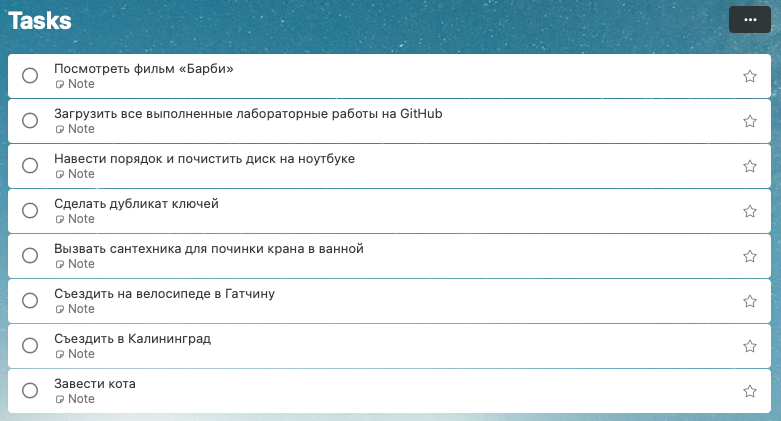
\includegraphics[width=0.9\textwidth]{images/tasks.png}}
  \caption{Список моих целей}
  \label{fig:task-list}
\end{figure}

\begin{figure}[H]
  \centering
  \fbox{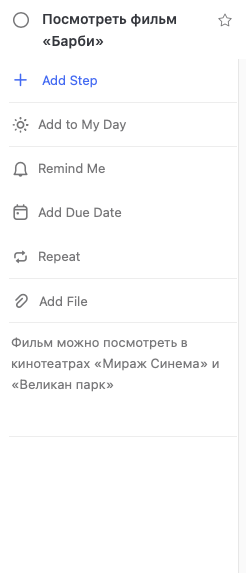
\includegraphics[width=0.23\textwidth]{images/task-1.png}}
  \fbox{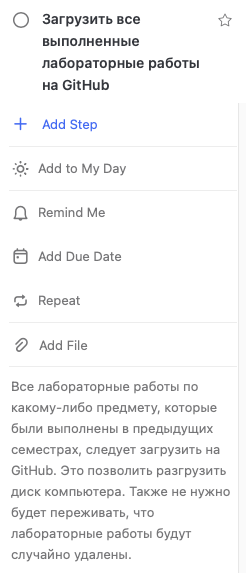
\includegraphics[width=0.23\textwidth]{images/task-2.png}}
  \fbox{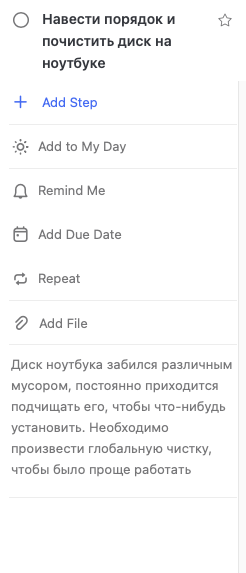
\includegraphics[width=0.23\textwidth]{images/task-3.png}}
  \fbox{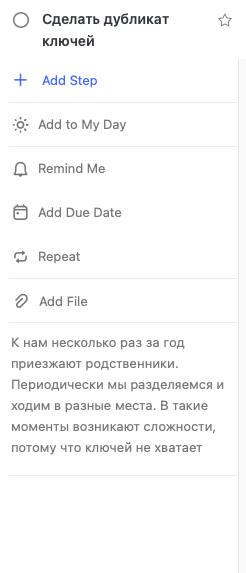
\includegraphics[width=0.23\textwidth]{images/task-4.png}}

  \vspace{1em}

  \fbox{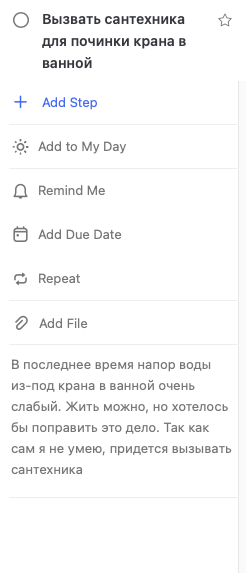
\includegraphics[width=0.23\textwidth]{images/task-5.png}}
  \fbox{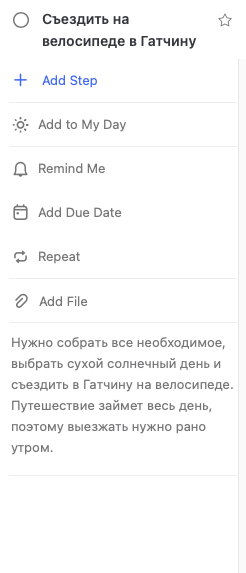
\includegraphics[width=0.23\textwidth]{images/task-6.png}}
  \fbox{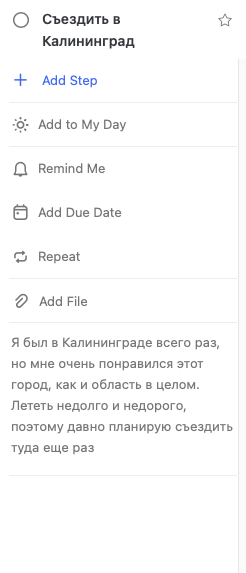
\includegraphics[width=0.23\textwidth]{images/task-7.png}}
  \fbox{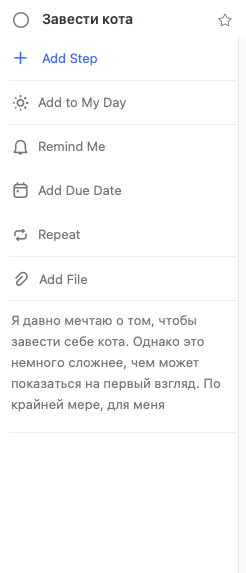
\includegraphics[width=0.23\textwidth]{images/task-8.png}}

  \caption{Описание целей}
  \label{fig:task-descriptions}
\end{figure}

\end{document}
